% Created by tikzDevice version 0.12.6 on 2026-08-03 03:41:06
% !TEX encoding = UTF-8 Unicode
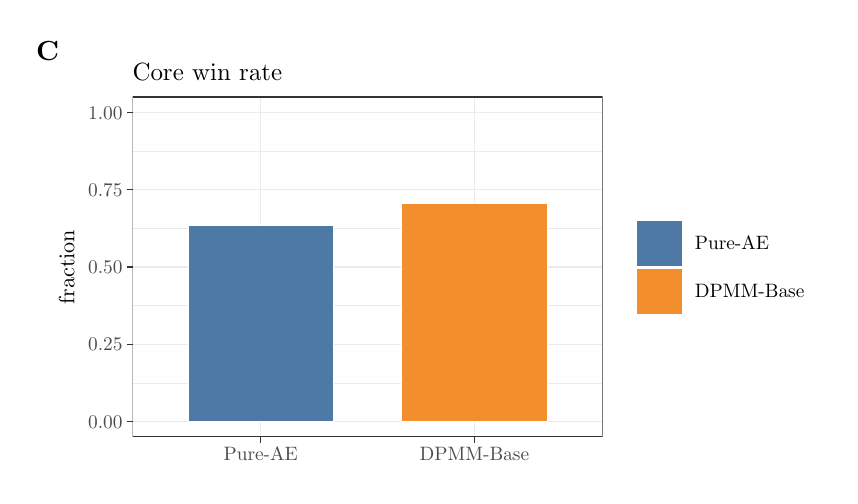
\begin{tikzpicture}[x=1pt,y=1pt]
\definecolor{fillColor}{RGB}{255,255,255}
\path[use as bounding box,fill=fillColor,fill opacity=0.00] (0,0) rectangle (289.70,161.83);
\begin{scope}
\path[clip] (  1.05,  1.74) rectangle (288.66,160.09);
\definecolor{drawColor}{RGB}{255,255,255}
\definecolor{fillColor}{RGB}{255,255,255}

\path[draw=drawColor,line width= 0.4pt,line join=round,line cap=round,fill=fillColor] (  1.05,  1.74) rectangle (288.66,160.09);
\end{scope}
\begin{scope}
\path[clip] ( 37.90, 13.93) rectangle (207.73,136.79);
\definecolor{fillColor}{RGB}{255,255,255}

\path[fill=fillColor] ( 37.90, 13.93) rectangle (207.73,136.79);
\definecolor{drawColor}{gray}{0.92}

\path[draw=drawColor,line width= 0.2pt,line join=round] ( 37.90, 33.48) --
	(207.73, 33.48);

\path[draw=drawColor,line width= 0.2pt,line join=round] ( 37.90, 61.40) --
	(207.73, 61.40);

\path[draw=drawColor,line width= 0.2pt,line join=round] ( 37.90, 89.32) --
	(207.73, 89.32);

\path[draw=drawColor,line width= 0.2pt,line join=round] ( 37.90,117.25) --
	(207.73,117.25);

\path[draw=drawColor,line width= 0.4pt,line join=round] ( 37.90, 19.52) --
	(207.73, 19.52);

\path[draw=drawColor,line width= 0.4pt,line join=round] ( 37.90, 47.44) --
	(207.73, 47.44);

\path[draw=drawColor,line width= 0.4pt,line join=round] ( 37.90, 75.36) --
	(207.73, 75.36);

\path[draw=drawColor,line width= 0.4pt,line join=round] ( 37.90,103.28) --
	(207.73,103.28);

\path[draw=drawColor,line width= 0.4pt,line join=round] ( 37.90,131.21) --
	(207.73,131.21);

\path[draw=drawColor,line width= 0.4pt,line join=round] ( 84.22, 13.93) --
	( 84.22,136.79);

\path[draw=drawColor,line width= 0.4pt,line join=round] (161.41, 13.93) --
	(161.41,136.79);
\definecolor{drawColor}{RGB}{255,255,255}
\definecolor{fillColor}{RGB}{242,142,43}

\path[draw=drawColor,line width= 0.3pt,fill=fillColor] (135.17, 19.52) rectangle (187.66, 98.26);
\definecolor{fillColor}{RGB}{78,121,167}

\path[draw=drawColor,line width= 0.3pt,fill=fillColor] ( 57.97, 19.52) rectangle (110.46, 90.55);
\definecolor{drawColor}{gray}{0.20}

\path[draw=drawColor,line width= 0.4pt,line join=round,line cap=round] ( 37.90, 13.93) rectangle (207.73,136.79);
\end{scope}
\begin{scope}
\path[clip] (  0.00,  0.00) rectangle (289.70,161.83);
\definecolor{drawColor}{gray}{0.30}

\node[text=drawColor,anchor=base east,inner sep=0pt, outer sep=0pt, scale=  0.70] at ( 34.30, 17.11) {0.00};

\node[text=drawColor,anchor=base east,inner sep=0pt, outer sep=0pt, scale=  0.70] at ( 34.30, 45.03) {0.25};

\node[text=drawColor,anchor=base east,inner sep=0pt, outer sep=0pt, scale=  0.70] at ( 34.30, 72.95) {0.50};

\node[text=drawColor,anchor=base east,inner sep=0pt, outer sep=0pt, scale=  0.70] at ( 34.30,100.87) {0.75};

\node[text=drawColor,anchor=base east,inner sep=0pt, outer sep=0pt, scale=  0.70] at ( 34.30,128.80) {1.00};
\end{scope}
\begin{scope}
\path[clip] (  0.00,  0.00) rectangle (289.70,161.83);
\definecolor{drawColor}{gray}{0.20}

\path[draw=drawColor,line width= 0.4pt,line join=round] ( 35.90, 19.52) --
	( 37.90, 19.52);

\path[draw=drawColor,line width= 0.4pt,line join=round] ( 35.90, 47.44) --
	( 37.90, 47.44);

\path[draw=drawColor,line width= 0.4pt,line join=round] ( 35.90, 75.36) --
	( 37.90, 75.36);

\path[draw=drawColor,line width= 0.4pt,line join=round] ( 35.90,103.28) --
	( 37.90,103.28);

\path[draw=drawColor,line width= 0.4pt,line join=round] ( 35.90,131.21) --
	( 37.90,131.21);
\end{scope}
\begin{scope}
\path[clip] (  0.00,  0.00) rectangle (289.70,161.83);
\definecolor{drawColor}{gray}{0.20}

\path[draw=drawColor,line width= 0.4pt,line join=round] ( 84.22, 11.93) --
	( 84.22, 13.93);

\path[draw=drawColor,line width= 0.4pt,line join=round] (161.41, 11.93) --
	(161.41, 13.93);
\end{scope}
\begin{scope}
\path[clip] (  0.00,  0.00) rectangle (289.70,161.83);
\definecolor{drawColor}{gray}{0.30}

\node[text=drawColor,anchor=base,inner sep=0pt, outer sep=0pt, scale=  0.70] at ( 84.22,  5.51) {Pure-AE};

\node[text=drawColor,anchor=base,inner sep=0pt, outer sep=0pt, scale=  0.70] at (161.41,  5.51) {DPMM-Base};
\end{scope}
\begin{scope}
\path[clip] (  0.00,  0.00) rectangle (289.70,161.83);
\definecolor{drawColor}{RGB}{0,0,0}

\node[text=drawColor,rotate= 90.00,anchor=base,inner sep=0pt, outer sep=0pt, scale=  0.80] at ( 16.86, 75.36) {fraction};
\end{scope}
\begin{scope}
\path[clip] (  0.00,  0.00) rectangle (289.70,161.83);
\definecolor{fillColor}{RGB}{255,255,255}

\path[fill=fillColor] (215.73, 54.02) rectangle (286.66, 96.71);
\end{scope}
\begin{scope}
\path[clip] (  0.00,  0.00) rectangle (289.70,161.83);
\definecolor{fillColor}{RGB}{255,255,255}

\path[fill=fillColor] (219.73, 75.36) rectangle (237.08, 92.71);
\definecolor{drawColor}{RGB}{255,255,255}
\definecolor{fillColor}{RGB}{78,121,167}

\path[draw=drawColor,line width= 0.3pt,fill=fillColor] (220.09, 75.72) rectangle (236.72, 92.35);
\end{scope}
\begin{scope}
\path[clip] (  0.00,  0.00) rectangle (289.70,161.83);
\definecolor{fillColor}{RGB}{255,255,255}

\path[fill=fillColor] (219.73, 58.02) rectangle (237.08, 75.36);
\definecolor{drawColor}{RGB}{255,255,255}
\definecolor{fillColor}{RGB}{242,142,43}

\path[draw=drawColor,line width= 0.3pt,fill=fillColor] (220.09, 58.37) rectangle (236.72, 75.01);
\end{scope}
\begin{scope}
\path[clip] (  0.00,  0.00) rectangle (289.70,161.83);
\definecolor{drawColor}{RGB}{0,0,0}

\node[text=drawColor,anchor=base west,inner sep=0pt, outer sep=0pt, scale=  0.70] at (241.08, 81.62) {Pure-AE};
\end{scope}
\begin{scope}
\path[clip] (  0.00,  0.00) rectangle (289.70,161.83);
\definecolor{drawColor}{RGB}{0,0,0}

\node[text=drawColor,anchor=base west,inner sep=0pt, outer sep=0pt, scale=  0.70] at (241.08, 64.28) {DPMM-Base};
\end{scope}
\begin{scope}
\path[clip] (  0.00,  0.00) rectangle (289.70,161.83);
\definecolor{drawColor}{RGB}{0,0,0}

\node[text=drawColor,anchor=base west,inner sep=0pt, outer sep=0pt, scale=  0.90] at ( 37.90,142.78) {Core win rate};
\end{scope}
\begin{scope}
\path[clip] (  0.00,  0.00) rectangle (289.70,161.83);
\definecolor{drawColor}{RGB}{0,0,0}

\node[text=drawColor,anchor=base,inner sep=0pt, outer sep=0pt, scale=  1.00] at (  7.20,150.08) {\bfseries C};
\end{scope}
\end{tikzpicture}
